

In the DARPA CASE project, a suite of tools were developed to help system engineers design cyber-physical systems that must satisfy cyber-resiliency requirements.
For demonstration, we modeled a UAV system. The target application is waterway monitor. The waterway area consists of a set of fly-in zones and fly-out zones. The goal of the UAV is to fly from one end of the waterway to the other end in minimum distance, while staying inside the fly-in zones and outside the fly-out zones.
 
Figure \ref{SW} shows an overview of the software architecture. The UAV software originally contains 5 threads: UxAS \cite{uxas}, waypoint plan manager, UART driver, radio driver, and fly zone database. They are associated with various levels of trustworthy. For example, the UxAS thread, used as a blackbox software component, was deemed as potentially security-compromised.
By applying the CASE tools, a list of security vulnerabilities were identified. Then the user was guided by the tools to invoke a series of model transformations to address the vulnerabilities. The transformation automatically inserted assurance components (8 threads): attestation gate, attestation manager, 2 monitors, and 4 filters. The verification goal is to prove that the key system security properties are satisfied after the transformation.

\begin{figure}[ht!]
\centering
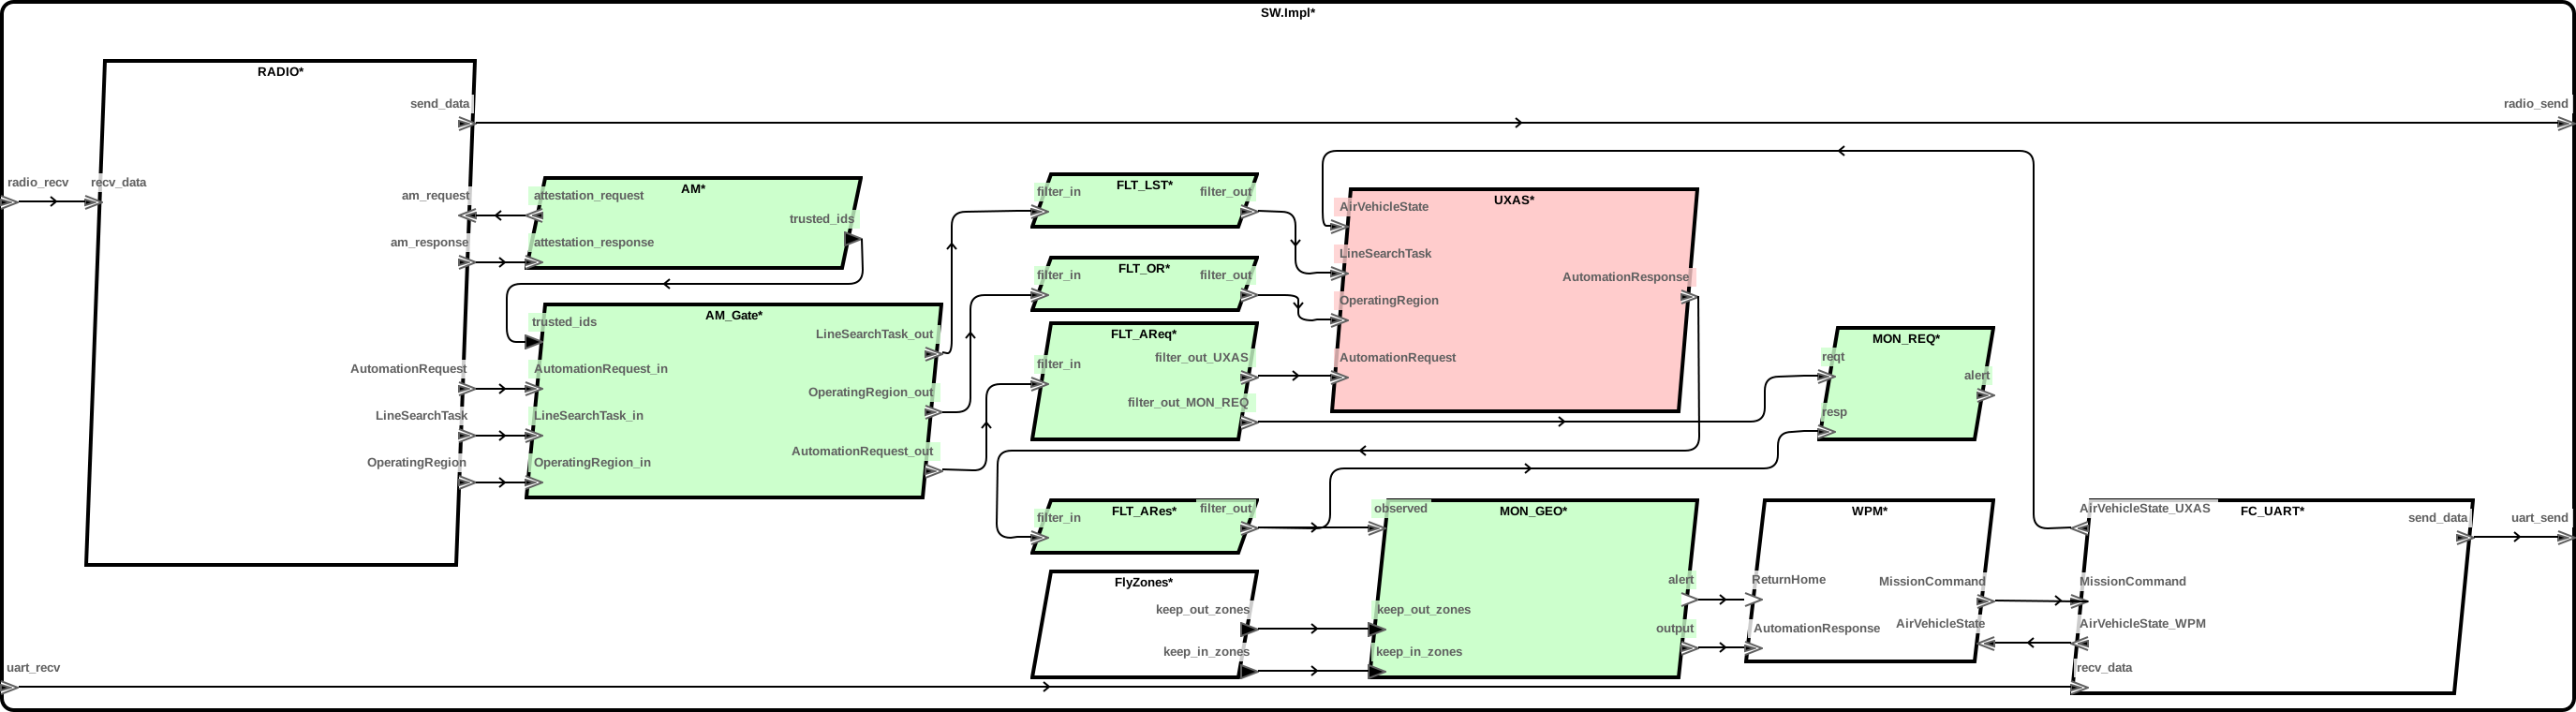
\includegraphics[width=120mm]{sw3.png}
\caption{A UAV Software Architecture Model in AADL \label{SW}}
\end{figure}

All 13 threads were mapped to the mission computer processor. The seL4 microkernel was chosen as part of the implementation platform. And an seL4 domain schedule was created. All threads are periodic with a period of 500 ms. Each thread is activated exactly once in the scheduling cycle. The allocated processor time for each thread ranges from 2 ms (filter/monitor) to 100 ms (UxAS).

Although in the AADL model, event and event data ports are mostly used, they are intended to model the event-triggered execution of periodic threads. 
Since each thread executes exactly once in every scheduling cycle, the number of queued events or data is always equal or less than one. 
Thus, the proposed modeling framework can be applied.

Four system-level security properties were created to ensure: 1) the output UART and RF messages are \emph{well-formed}; 2) the system only responds to trusted sources; 3) the waypoints generated are \emph{geo-fenced}. The properties were proved in less than 2 minutes on a PC with 2.6 GHz CPU and 32 GB RAM.

